\section{Puppet}
Puppet là một framework mã nguồn mở và là công cụ để quản lý cấu hình của hệ thống máy tính. Trong phần này, chúng ta sẽ tìm hiểu tổng quan về Puppet: cách thức nó hoạt động, cách nó quản lý cấu hình của hệ thống máy chủ, cách cài đặt chúng trên các nền tảng khác nhau. Tiếp đó, chúng ta sẽ tìm hiểu kiến trúc của Puppet, cách Puppet thu thập và quản lý các gói dữ liệu cấu hình.

\subsection{Tổng quan về Puppet}
Puppet là một công cụ quản lý cấu hình mã nguồn mở viết bằng Ruby, được sử dụng để quản lý cấu hình máy chủ và tự động hóa hệ thống trong các trung tâm dữ liệu của Google, Twitter, thị trường chứng khoán New York, và nhiều doanh nghiệp lớn khác. Puppet được phát triển đầu tiên bởi Puppet Labs, và hiện tại Puppet Labs cũng là người duy trì chính của dự án này. Puppet được dùng để quản lý có khi chỉ vài máy chủ nhưng cũng có khi lên tới 50.000 máy chủ, cùng với đó là đội quản trị hệ thống từ một người tới hàng trăm người.

Puppet là một công cụ để quản lý cấu hình và bảo trì hệ thống máy tính; ngôn ngữ cấu hình của nó rất đơn giản. Chúng ta chỉ cần chỉ cho Puppet thấy chúng ta muốn cấu hình máy tính của chúng ta như thế nào, nó sẽ thực hiện đúng những gì chúng ta muốn. Khi hệ thống có sự thay đổi chẳng hạn như một phiên bản cập nhật của gói phần mềm, thêm người dùng mới hay một cấu hình nào đó thay đổi, Puppet tự động cập nhật tất cả các máy chủ trong hệ thống đúng như cấu hình chúng ta muốn.

\begin{figure}[htb]
    \begin{center}
    \fbox{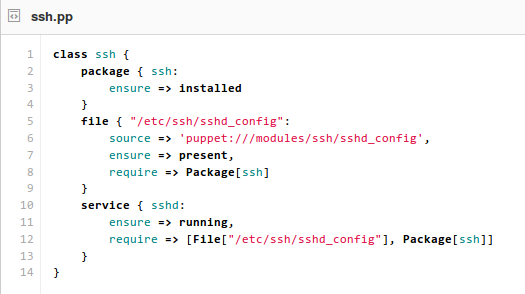
\includegraphics[width=0.9\textwidth]{images/puppet_ssh_pp.png}}
    \end{center}
    \caption{Ví dụ về ngôn ngữ cấu hình của Puppet}
    \label{fig:puppet_ssh_pp}
\end{figure}

Như hình vẽ trên, Puppet đảm bảo rằng gói phần mềm \textbf{\textit{ssh}} được cài đặt và file cấu hình dịch vụ SSH \footnote{Secure Shell: \url{https://en.wikipedia.org/wiki/Secure_Shell}} \textbf{\textit{/etc/ssh/sshd\_config}} của tất cả các máy chủ trong hệ thống mà Puppet quản lý đều có cùng nội dung mới file đã định trước; thêm vào đó, Puppet đảm bảo việc dịch vụ này luôn được chạy giúp người quản trị hệ thống có thể can thiệp thủ công khi cần thiết.

\subsection{Kiến trúc của Puppet}

Puppet được xây dựng với hai chế độ làm việc:

\begin{itemize}
\item \textbf{Chế độ client/server} Có một máy chủ trung tâm với một dịch vụ chạy nền kết nối đến các "agents" chạy độc lập trên các máy trạm.

\item \textbf{Chế độ serverless} Chỉ có một tiến trình duy nhất thực hiện tất cả các công việc.
\end{itemize}

Để đảm bảo tính nhất quán giữa các chế độ, Puppet luôn có sự minh bạch trong các liên kết nội bộ của bản thân nó. Do đó, hai chế độ này sử dụng cùng một đường dẫn như nhau cho dù chúng có giao tiếp với nhau qua mạng hay không. Mỗi lệnh được thực thi cho dù lấy cấu hình từ bản nó hay một máy khác ở xa trong mạng thì chúng đều có một cách thực hiện như nhau. Tuy nhiên cũng phải lưu ý rằng, chế độ serverless là một phần trong trong mô hình client/server: tất cả các file cấu hình sẽ được đẩy xuống cho agents ở máy trạm xử lý, tại đây máy trạm chạy ở chế độ serverless sẽ làm việc trực tiếp với các tệp tin cấu hình và thực thi chúng. Phần này sẽ chỉ tập trung vào chế độ client/server bởi vì nó dễ hiểu hơn với các thành phân riêng biệt, nhưng hãy luôn nhớ rằng tất cả đều chạy ở chế độ serverless.

Một trong những lựa chọn ngay từ đầu trong kiến trúc của Puppet là máy trạm không nên truy cập trực tiếp (raw access) vào các module, thay vào đó, chúng lấy các cấu hình đã được chuẩn bị sẵn từ trước. Việc này cung cấp nhiều lợi ích:

\begin{itemize}
\item \textbf{Thứ nhất}, chung ta thực hiện được việc tối thiểu quyền hạn cần thiết. Trong đó mỗi máy chủ chỉ biết chính xác những gì nó cần phải biết (nó nên được cấu hình như thế nào), nhưng nó không biết (và không quan tâm) những máy trạm khác được cấu hình như thế nào.

\item \textbf{Thứ hai}, chúng ta hoàn toàn có thể phân tách các quyền cần thiết để tạo ra một cấu hình (bao gồm cả quyền truy cập vào nơi lưu trữ dữ liệu trung tâm) mà nó sẽ được thực hiện dưới máy trạm.

\item \textbf{Thứ ba}, chúng ta có thể chạy các máy trạm trong chế độ ngắt kết nối với máy chủ trung tâm, nhưng các cấu hình đã có của Puppet sẽ vẫn luôn được áp dụng. Nghĩa là, cho dù máy chủ trung tâm (puppet-master) không còn hoạt động hoặc không có kết nối đến nó thì mỗi máy trạm vẫn có thể làm việc độc lập.

\end{itemize}

Với sự lựa chọn này, quy trình làm việc trở nên tương đối đơn giản

\begin{itemize}
\item Tiến trình trên máy trạm (Puppet agent) thu thập các thông tin về hệ thống mà nó đang làm việc, sau đó chuyển các thông tin này tới máy chủ trung tâm (Puppet Master)

\item Tại máy chủ trung tâm, các thông tin đó cùng các module trên ổ đĩa cục bộ được biên dịch thành một cấu hình cho một máy chủ cụ thể và trả lại nó cho các tiến trình trên máy trạm.

\item Các tiến trình trên máy trạm áp dụng những cấu hình cục bộ này và nó chỉ ảnh hưởng tới riêng máy trạm đó. Sau đó, các tập tin báo cáo được tạo ra rồi đưa kết quả về máy chủ trung tâm.
\end{itemize}

\begin{figure}[h!]
    \begin{center}
    \fbox{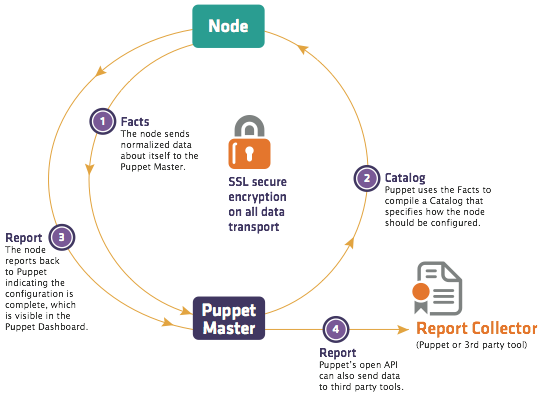
\includegraphics[width=0.9\textwidth]{images/puppet_dataflow.png}}
    \end{center}
    \caption{Biểu đồ luồng dữ liệu của Puppet}
    \label{fig:puppet_dataflow}
\end{figure}

Vì thế, các agent có quyền truy cập vào thông tin riêng trên hệ thống của mình, các cấu hình của nó, cũng như các báo cáo nó tạo ra. Máy chủ trung tâm có bảo sao của tất cả các dữ liệu này, cùng với quyền truy cập toàn bộ các module, cũng như bất kỳ cơ sở dữ liệu và dịch vụ nào khác dùng để biên dịch các cấu hình cần thiết.

Ngoài các thành phần ở trong quy trình làm việc này, có rất nhiều loại dữ liệu được Puppet sử dụng cho các giao tiếp nội bộ của nó. Các loại dữ liệu rất quan trọng, bởi vì chúng hoàn thực hiện tất cả các thông tin liên lạc, đồng thời chúng cũng cung cấp các giao diện công cộng cho những công cụ khác sử dụng hay làm việc với chúng.

\newpage
\clearpage

\begin{figure}[h!]
    \begin{center}
    \fbox{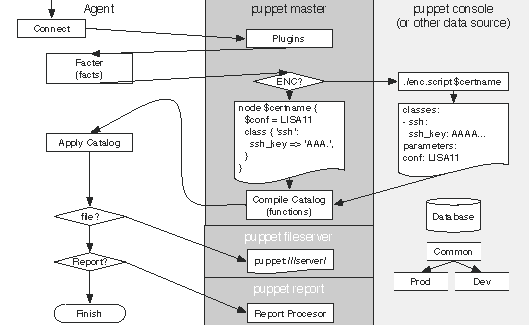
\includegraphics[width=0.9\textwidth]{images/puppet_timing_diagram.png}}
    \end{center}
    \caption{Luồng dữ liệu lưu chuyển \\ giữa các thành phần và tiến trình của Puppet}
    \label{fig:puppet_timing_diagram}
\end{figure}

Các kiểu dữ liệu quan trọng nhất trong Puppet là:

\begin{itemize}
\item \textbf{Facts}: Thu thập các thông thin hệ thống trên mỗi máy trạm. Những thông tin này được dùng để biên dịch ra các cấu hình.

\item \textbf{Manifest}: Các tập tin chứa ngôn ngữ cấu hình Puppet, chúng thường được tổ chức thành các bộ sưu tập được gọi là module.

\item \textbf{Catalog}: Một đồ thị về các tài nguyên của máy chủ được quản lý và các rằng buộc giữa chúng.

\item \textbf{Report}: Tập hợp tất cả các sự kiện được tạo ra trong suốt quá trình tạo ra các Catalog.
\end{itemize}

Ngoài Facts, Manifests, Catalogs, and Reports, Puppet còn hỗ trợ các kiểu dữ liệu như các tệp tin, các chứng chỉ (được dùng trong việc xác thực) cùng nhiều kiểu dữ liệu khác.

\begin{figure}[h!]
    \begin{center}
    \fbox{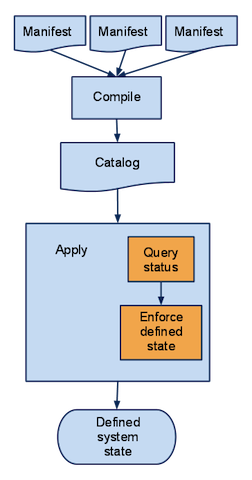
\includegraphics[scale=1.0]{images/puppet_manifest_to_defined_state_unified.png}}
    \end{center}
    \caption{Cách Puppet biên dịch và thực hiện một manifest\\ trong chế độ Serverless}
    \label{fig:puppet_dataflow}
\end{figure}

\begin{figure}[h!]
    \begin{center}
    \fbox{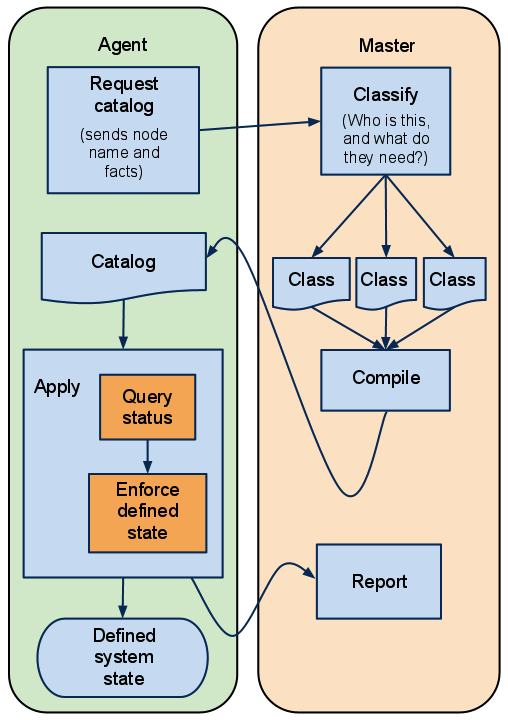
\includegraphics[width=0.85\textwidth]{images/puppet_manifest_to_defined_state_split.png}}
    \end{center}
    \caption{Cách Puppet biên dịch và thực hiện một manifest\\ trong chế độ Client-Server}
    \label{fig:puppet_dataflow}
\end{figure}

\clearpage
\subsection{Các thành phần của Puppet}

